\section{\bt{Introduction}{引言}}
\label{sec:introduction}

\bi{Enterprise databases and warehouses support recurring reporting, ad hoc analysis, and prediction. LLM-based data agents perform these tasks for different users in separate sessions~\cite{lei2025spider2,guo2024dsagent,liu2026agents}. Many questions share database-specific metric definitions, grain, filters, and joins~\cite{floratou2024nl2sql,robinson2024relbench}: monthly and quarterly reports can use the same revenue calculation over different periods (Figure~\ref{fig:metric-record}). Once established, this calculation should serve subsequent agents. Keeping it in session histories or private memories instead makes other agents repeat exploration or reconstruct it.}
{企业数据库与数据仓库支持反复出现的报表、即席分析与预测任务。大模型数据智能体通过独立会话为不同用户执行这些任务~\cite{lei2025spider2,guo2024dsagent,liu2026agents}。许多问题共用数据库特定的指标定义、粒度、过滤和连接~\cite{floratou2024nl2sql,robinson2024relbench}：月报与季报可以在不同期间使用相同的营业额计算（图~\ref{fig:metric-record}）。已确定的计算应当服务于后续智能体；若只保存在会话历史或私有记忆中，其他智能体仍需重复探索或重建计算。}

\begin{figure}[t]
\centering
% Vector drawing generated by tools/figures/metric_record.py from the 10-01 workload traces; rerun it after changing the figure.
\ifbilingual
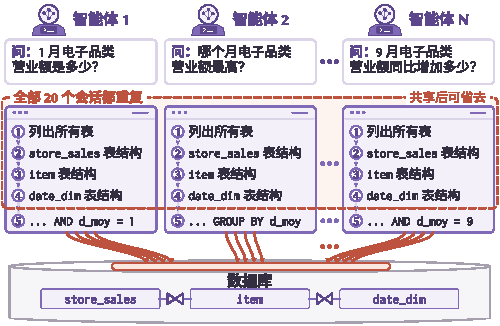
\includegraphics[width=\columnwidth]{figures/metric-record-zh}%
\else
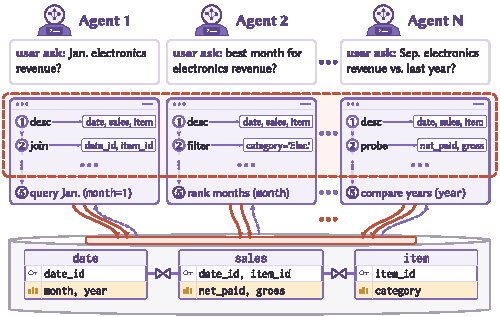
\includegraphics[width=\columnwidth]{figures/metric-record}%
\fi
\caption{\bt{Three agents asking about electronics revenue on the same database. Every session repeats steps 1--4; only the date filter in step~5 differs.}{同一数据库上询问电子品类营业额的三个智能体。每个会话都重复第 1--4 步，只有第 5 步的日期条件不同。}}
\label{fig:metric-record}
\Description{Three agent boxes, Agent 1, Agent 2 and Agent N, each show a question after the word ask: electronics revenue in January; which month had the highest electronics revenue; September electronics revenue versus a year earlier. An ellipsis between Agent 2 and Agent N marks more agents. Below them, one dashed box labelled repeated in all \WxSessions\ sessions and avoidable with sharing holds the same four steps for every agent: 1 list tables, 2 store\_sales schema, 3 item schema, 4 date\_dim schema. Under the box, each agent's step 5, final SQL, shows only its date filter: AND d\_moy = 1; GROUP BY d\_moy ORDER BY revenue DESC; AND d\_moy = 9 with GROUP BY d\_year, d\_moy.}
\end{figure}


\bi{Database changes can invalidate a shared calculation's assumptions. A revenue query may join sales to a lookup table on a previously unique key; a later load can introduce duplicate keys, causing double counting even though the SQL still executes. Rerunning it on fresh data preserves the error, whereas appending sales need not change the calculation. Maintenance must distinguish answer-changing updates from assumption-breaking changes, whose errors can propagate to every agent reusing the definition.}
{数据库变化可能破坏共享计算的前提。营业额查询可能按原本唯一的键连接销售表与查找表；后续装载引入重复键后，即使 SQL 仍能执行，也会重复计数。在新数据上重跑不能修复这一错误，而追加销售记录未必改变计算。维护因此需要区分改变答案的更新与破坏计算前提的变化，后者的错误可能传播到复用该定义的所有智能体。}

\bi{Agent memories retain and refine insights and workflows~\cite{zhao2024expel,wang2025awm,zhang2026ace}, and multi-agent memories share experience~\cite{zhang2025gmemory}. AgentSM reuses structured trajectories and composite database tools~\cite{biswal2026agentsm}; other systems extract script logic~\cite{weng2025datalab} or centralize metric definitions for SQL generation~\cite{dbt2026metricflow,databricks2026metricviews}. Continued reuse additionally requires checking whether data-dependent assumptions still hold. Task-feedback updates and shared execution alone do not establish this validity. We maintain learned computations through explicit conditions and dependencies, identifying affected knowledge and maintaining it for all consumers.}
{智能体记忆保留并改进洞见与工作流~\cite{zhao2024expel,wang2025awm,zhang2026ace}，多智能体记忆共享经验~\cite{zhang2025gmemory}。AgentSM 复用结构化轨迹与复合数据库工具~\cite{biswal2026agentsm}；其他系统提取脚本逻辑~\cite{weng2025datalab}，或集中管理指标定义以生成 SQL~\cite{dbt2026metricflow,databricks2026metricviews}。持续复用还需要检查数据前提是否仍然成立，仅根据任务反馈更新记忆或执行共享定义不能确立这种有效性。我们通过显式条件与依赖维护学得的计算，定位受影响的知识，并面向全部使用者统一维护。}

\bi{Three challenges follow. \emph{Extracting reusable computation} requires separating business logic from question parameters and recording reuse assumptions. \emph{Localizing maintenance} requires identifying affected conditions, revalidating changed dependencies, and repairing definitions while retaining valid knowledge: a dependency change need not invalidate its computation. \emph{Coordinating validation and reuse} requires sharing checks across agents and ensuring that evidence from an earlier state still applies to the consuming query's data.}
{这一问题带来三项挑战。\emph{提取可复用计算}需要分离业务逻辑与问题参数，并记录复用前提。\emph{定位维护范围}需要识别受影响的条件、重验变化的依赖，并在保留有效知识的同时修复定义：依赖变化未必使计算失效。\emph{协调验证与复用}需要跨智能体共享检查，并确认先前状态上的证据仍适用于消费查询实际读取的数据。}

\bi{We present \system\ (\textbf{M}etric-\textbf{A}ware \textbf{V}alidation and \textbf{R}euse for \textbf{A}gents), a shared memory layer between heterogeneous data agents and the database. It manages \emph{executable definitions with checkable reuse conditions}. Metrics separate measures, grain, joins, and filters from question parameters; features additionally identify entities and temporal windows. Deterministic publication checks validate definitions and compare compiled results with verified metric answers or submitted feature values. Later agents instantiate accepted definitions for new periods or prediction instances.}
{本文提出 \system{}（\textbf{M}etric-\textbf{A}ware \textbf{V}alidation and \textbf{R}euse for \textbf{A}gents），一个位于异构数据智能体与数据库之间的共享记忆层。它共同管理\emph{可执行定义与可检查的复用条件}。指标将度量、粒度、连接和过滤与问题参数分离；特征进一步记录实体与时间窗口。确定性发布检查验证定义，并将编译结果与核实的指标答案或提交的特征值比较。后续智能体为新的期间或预测样本实例化已通过检查的定义。}

\bi{Condition identities and dependency versions let consumers share validation evidence and locate checks requiring renewal. Failed conditions trigger repair or invalidation of affected metrics while valid knowledge remains available. Validated repairs serve subsequent consumers, avoiding repeated correction. Metric validation and execution use the same database snapshot, extending shared work from initial discovery to continued maintenance.}
{条件标识与依赖版本使使用者共享验证证据，并定位需要更新的检查。条件失败时，系统修复受影响的指标或将其标记为不可复用，同时保留有效知识。通过验证的修复服务于后续使用者，避免重复纠正。指标验证与执行使用同一数据库快照，将共享工作从最初的知识发现延伸到持续维护。}

\bi{Our contributions are:}
{本文的主要贡献如下：}
\begin{itemize}
\item \bi{We implement \system, a shared database memory layer that makes knowledge from individual sessions reusable across heterogeneous agents, tasks, and sessions.}
{我们实现了共享数据库记忆层 \system，使单个会话获得的知识能够跨异构智能体、任务和会话复用。}

\item \bi{We extract parameterized, executable metric and feature definitions from successful sessions, separating reusable computation from task inputs, recording reuse conditions, and checking candidates before publication.}
{我们从成功会话中提取参数化的可执行指标与特征定义，分离可复用计算与任务输入，记录复用条件，并在发布前检查候选。}

\item \bi{We develop dependency-aware validation and repair that rechecks affected conditions, blocks metric reuse when required conditions fail on the query snapshot, preserves unaffected knowledge, and shares validated repairs.}
{我们设计基于依赖的验证与修复，重验受影响的条件，阻止复用在查询快照上不满足所需条件的指标，保留未受影响的知识，并共享通过验证的修复。}

\item \bi{We evaluate \system\ on RelBench and five analytical schemas against agent memories, feature-engineering systems, and maintenance policies, measuring cross-agent reuse, correctness under eleven data changes, quality, tokens, and end-to-end time, including learning, publication, validation, and maintenance costs.}
{我们在 RelBench 与五种分析模式上，将 \system 与智能体记忆、特征工程系统及维护策略比较，测量跨智能体复用、十一种数据变化后的正确性、质量、token 与端到端耗时，并计入学习、发布、验证和维护的开销。}
\end{itemize}
